\documentclass[PICOAPC.tex]{subfiles}
\newcommand\pdeg{.\!\!\degree}
\newcommand\parcm{.\!\!'}

\section{Technical Overview}
\label{sec:techoverview}

\vspace{-0.06in}

PICO meets all of its science-driven instrument requirements with a single instrument: an imaging polarimeter with 21 logarithmically spaced frequency bands centered between 21 and 799\,GHz (Table~\ref{tab:spec_bands}). The instrument has a two-reflector Dragone-style telescope; see Figure~\ref{fig:InstrumentCAD}. The focal plane is populated by \ac{TES} bolometers and read out using a time-domain multiplexing scheme. The instrument has both passive and active cooling stages. PICO operates from the Earth-Sun L2 and employs a single science observing mode, providing highly redundant coverage of the full sky. A full description of the reference design is given by \citet{pico_report}.

\begin{figure}[h] 
\hspace{-0.1in}
\parbox{4.8in}{\centerline{
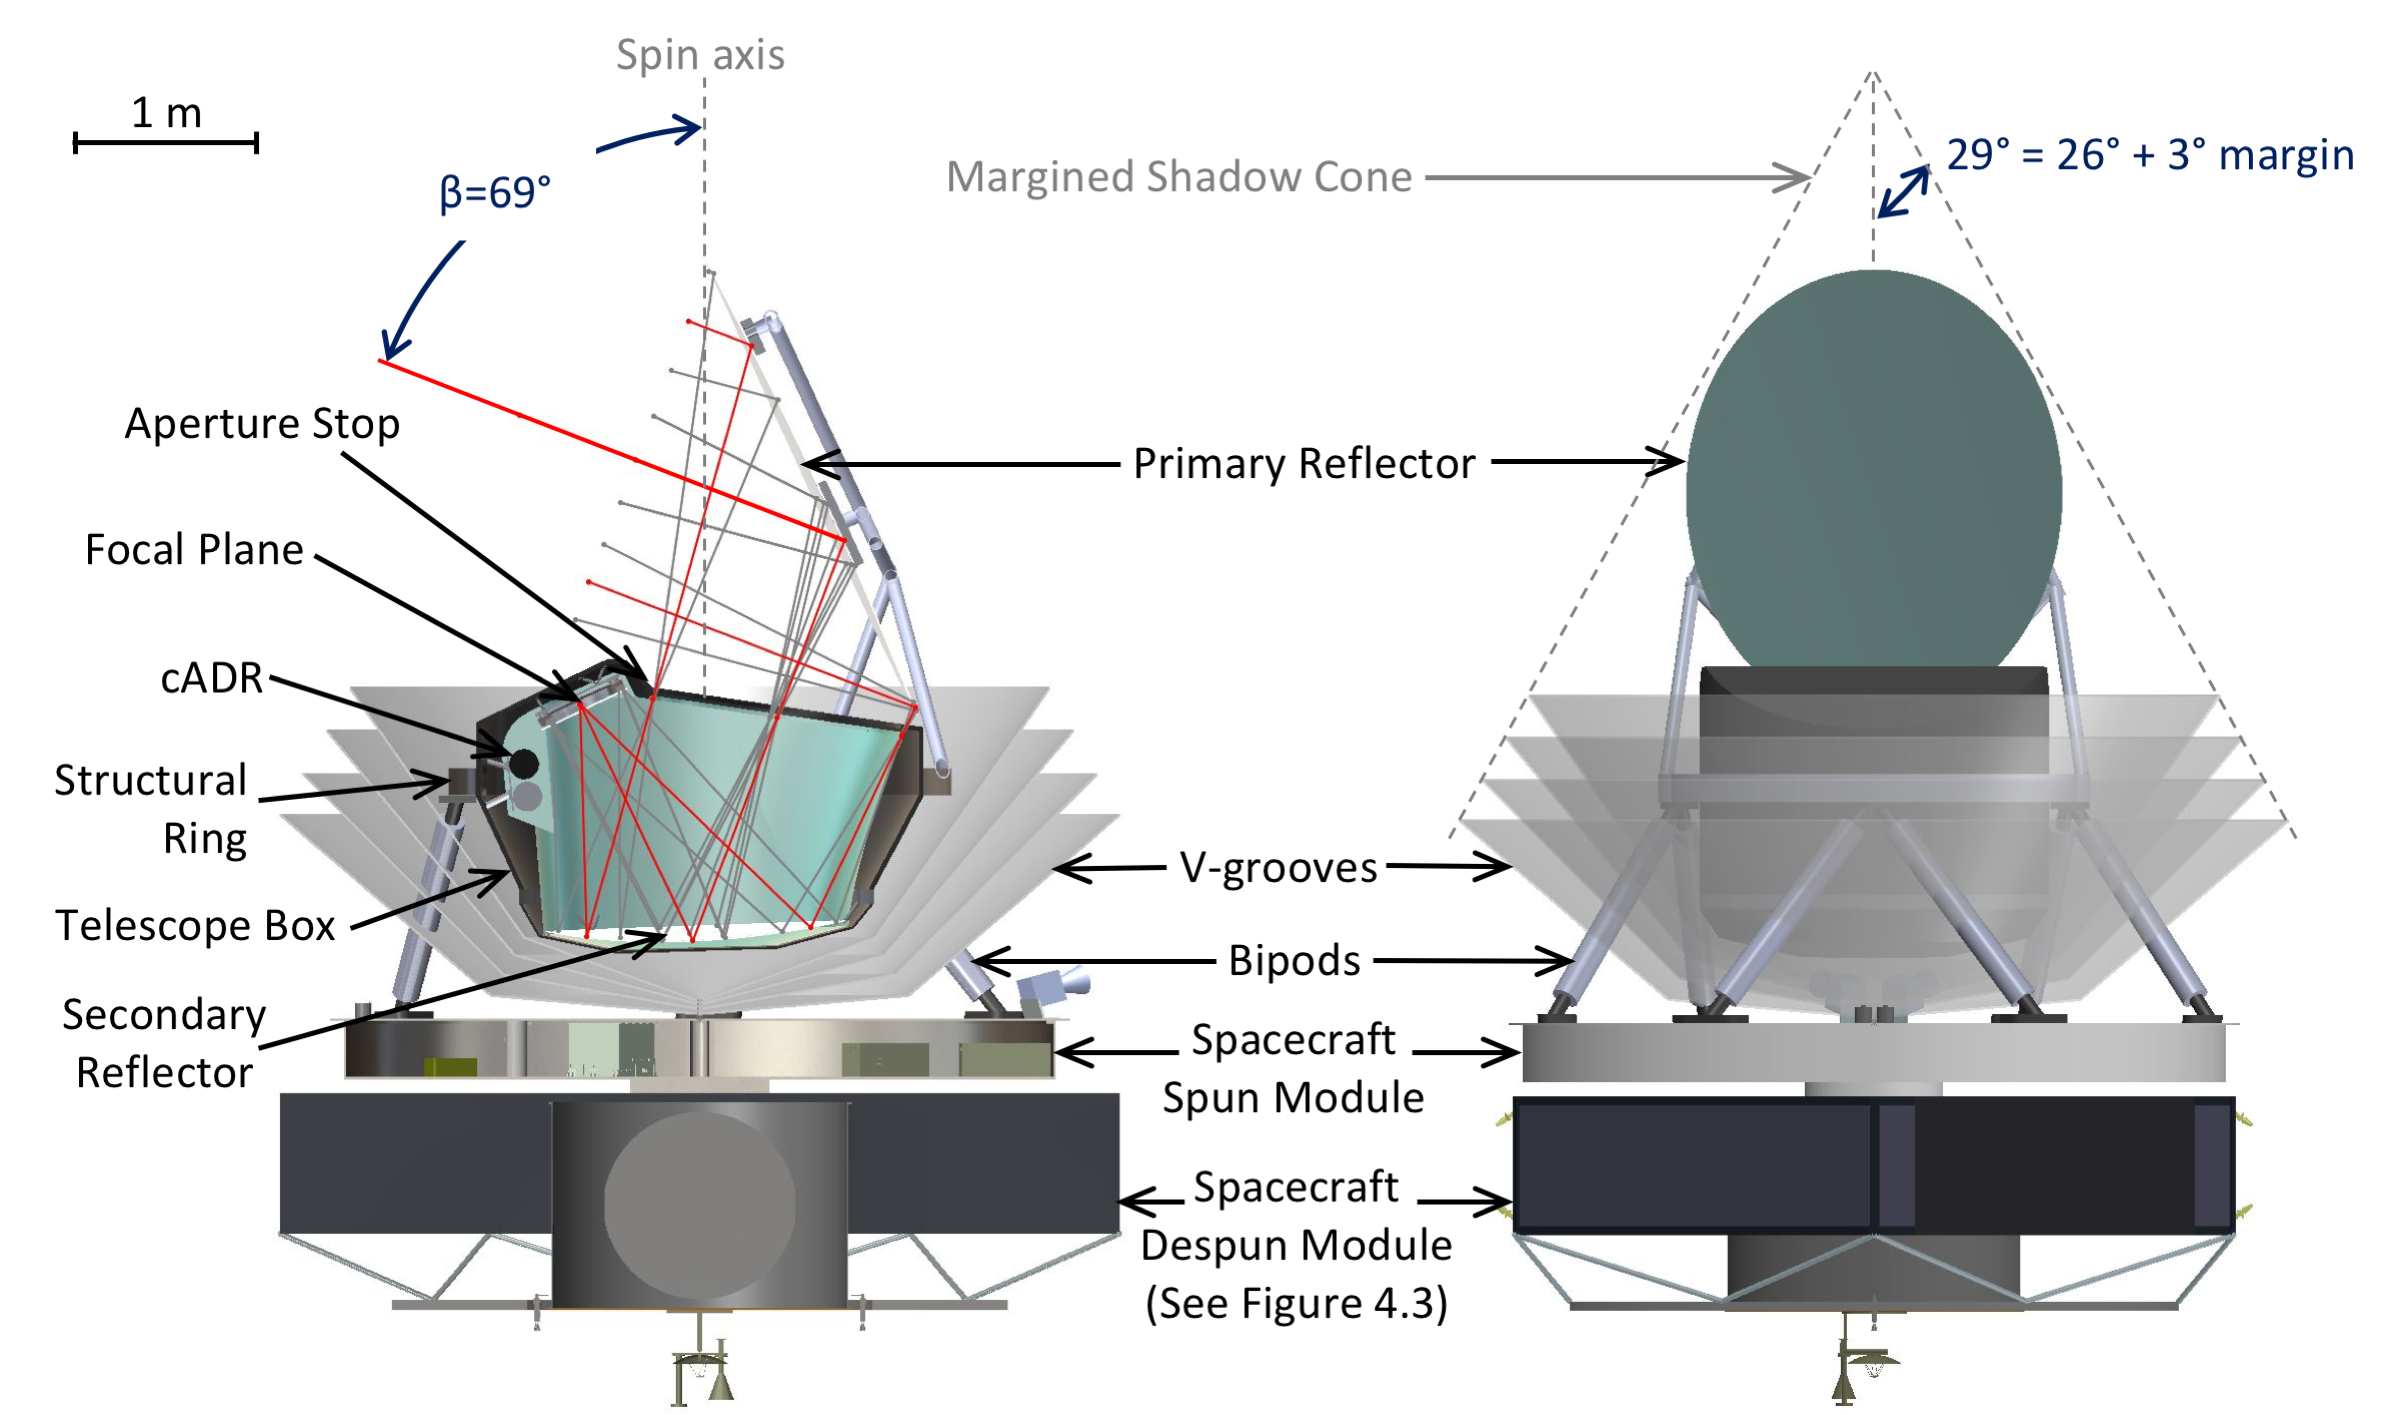
\includegraphics[width=4.8in]{figures/InstrumentCAD.png} }}
\hspace{0.0in}
\parbox{1.6in}{
\caption{\captiontext
PICO overall configuration in side view and cross section (left), and front view with V-Groove assembly shown semi-transparent (right).  The mission consists of a single science instrument mounted on a structural ring. The ring is supported by bipods on a stage spinning at 1~RPM relative to a despun module. Only power and digital information pass between the spun and despun stages. 
\label{fig:InstrumentCAD}} }
%\end{center}
\vspace{-0.15in}
\end{figure}

\vspace{-0.06in}

\subsection{Telescope, Detectors, and Readout}
\label{sec:telescope} 

\vspace{-0.03in}


The PICO 1.4~m aperture, two-mirror telescope gives a large diffraction-limited field of view, sufficient to support approximately $10^4$ detectors; arcminute resolution at 800\,GHz; low instrumental and cross-polarization; and low sidelobe response. There are no moving parts in the PICO optical system, reducing mission risk. There are no lenses, eliminating absorption and reflection losses and obviating the need for developing broad-band anti-reflection coatings. The primary mirror is passively cooled to $\sim$20~K. An aperture stop and a secondary mirror are actively cooled to 4.5~K. 

%The sensitivity of PICO's detectors is limited by irreducible backgrounds: the CMB at frequencies below 400~GHz, and emission from the cold primary mirror at higher frequencies. Therefore, the required sensitivity determines the detector count in each band. 
The PICO focal plane has a total of 12,996 \ac{TES} detectors, 175~times the number flown aboard \planck . The required full-sky, 5-year survey depth is 0.87~$\mu$K\,arcmin; the current best estimate performance is 0.61~$\mu$K\,arcmin, offering 40\% noise margin. PICO is the most sensitive CMB experiment proposed for the next decade. To achieve similar raw sensitivity, a ground-based instrument would require $\simgt$50 times the number of detectors. 

%\begin{wraptable}[13]{r}{0.43\textwidth}
%\vskip -2mm
%\hskip1.4cm
%\begin{minipage}[t]{0.3\textwidth}
%\caption{\textbf{Mission Parameters}\label{tab:specs}}
%\begingroup
%%\openup 5pt
%\newdimen\tblskip \tblskip=5pt
%\nointerlineskip
%\vskip -7mm
%\footnotesize %\footnotesize
%\setbox\tablebox=\vbox{
%    \newdimen\digitwidth
%    \setbox0=\hbox{\rm 0}
%    \digitwidth=\wd0
%    \catcode`*=\active
%    \def*{\kern\digitwidth}
%%
%    \newdimen\signwidth
%    \setbox0=\hbox{+}
%    \signwidth=\wd0
%    \catcode`!=\active
%    \def!{\kern\signwidth}
%%
%\halign{%
%\hbox to 1.4in{#\leaderfil}\tabskip=0.6em plus 0.6em&
%#\hfil\tabskip=0pt\cr
%\noalign{\doubleline}
%\multispan2 Full sky CMB polarization map depth$^{a}$ :\hfil\cr
%\quad Baseline&0.87 $\mu$K$_{\rm CMB}$ arcmin\cr
%\hskip1.75cm equivalent to 3300 \textit{Planck} missions\cr
%\quad CBE$^{b}$&0.61 $\mu$K$_{\rm CMB}$ arcmin\cr
%\hskip1.75cm equivalent to 6400 \textit{Planck} missions\cr
%Survey duration / start & 5\,yrs / 2029 \cr
%Orbit type & Sun-Earth L2 \cr
%Launch mass & 2147\,kg \cr
%Total power &1320\,W \cr
%Data rate & 6.1\,Tbits/day \cr
%Cost&\$\,958M\cr
%%Launch&2029\cr
%\noalign{\vskip 5pt\hrule\vskip 3pt}
%\noalign{$^{a}$ rms noise in $1\times1$ arcmin$^{2}$ pixel.} % footnote to table
%\noalign{$^{b}$ CBE = Current best estimate.} % footnote to table
%} % close halign
%} % close vbox
%\endPlancktable
%\endgroup
%%\end{table}
%\end{minipage}

%\end{wraptable}

% Start second table
%\vskip0.5cm
%\hskip0.2cm

\begin{wraptable}[24]{r}{0.43\textwidth}
\vskip -2mm
%\hskip1.4cm
\begin{minipage}[t]{0.4\textwidth}
\footnotesize
\caption{\textbf{Frequency Bands, Resolution, and Noise Level}\label{tab:spec_bands}}
\vskip -2mm
\begin{tabular}{|c|c|c|c|}
\hline
Frequency& FWHM& \multicolumn{2}{c|}{Polarization map depth}  \\ 
\cline{3-4}
& & Baseline & CBE  \\
 \space [GHz] & [arcmin]  & [$\mu$K$_{\rm CMB}$]$^{a}$ & [$\mu$K$_{\rm CMB}]^{a}$ \\ \hline
21 & 38.4 & 23.9 & 16.9 \\ 
25 & 32.0 & 18.4 & 13.0 \\ 
30& 28.3 & 12.4 & 8.7 \\ 
36& 23.6 & 7.9 & 5.6 \\ 
43& 22.2 & 7.9 & 5.6 \\ 
52& 18.4 & 5.7 & 4.0 \\ 
62& 12.8 & 5.4 & 3.8 \\ 
75& 10.7 & 4.2 & 3.0 \\ 
90 & 9.5 & 2.8 & 2.0 \\ 
108 & 7.9 & 2.3 & 1.6\\ 
129 & 7.4 & 2.1 & 1.5 \\ 
155 & 6.2 & 1.8 & 1.3 \\ 
186 & 4.3 & 4.0 & 2.8 \\ 
223 & 3.6 & 4.5 & 3.2 \\ 
268 & 3.2 & 3.1 & 2.2 \\ 
321 & 2.6 & 4.2 & 3.0 \\ 
385 & 2.5 & 4.5 & 3.2 \\ 
462 & 2.1 & 9.1 & 6.4 \\ 
555 & 1.5 & 45.8 & 32.4 \\ 
666 & 1.3 & 177 & 125 \\ 
799 & 1.1 & 1050 & 740 \\ 
\noalign{\vskip 0pt\hrule\vskip 3pt}
\noalign{$^{a}$ For values in [Jy/sr] units see~\citet{pico_report}.} % footnote to table

\end{tabular}

%\end{table}
\end{minipage}
\end{wraptable}


There is broad flexibility in the detailed implementation of the PICO focal plane. In the baseline design we employ three-color sinuous antenna/lenslet pixels~\citep{Suzuki2014} for the 21--462\,GHz bands, and single color, feedhorn-coupled, polarization sensitive bolometers for the three higher frequency bands. PICO can also achieve its required performance with two-color pixels~\citep{nist_design} (for 21--462~GHz) with a total of 19 bands and the same noise margin, or even with single-color pixels at all 21 bands~\citep{bicep_design} and 17\% noise margin. Current Ground-based instruments use all three technologies at a narrower range of frequencies. There are funding mechanisms and development programs in place to adapt the technologies to a broader ranger of frequencies and to space applications; see Section~\ref{sec:techdrivers}. 

%PICO can achieve its required performance with other already focal plane technologies  than albeit with reduce
%Niobium microstrips mediate the signals between the antenna and detectors, and partition the wide continuous bandwidth into three narrow channels using integrated, on-wafer, micro-machined filter circuits~\citep{OBrient2013}. Six transition edge sensor bolometers per pixel detect the radiation in two orthogonal polarization states. 

%PICO's highest three frequency channels are beyond the niobium superconducting band-gap, rendering on-wafer, microstrip filters a poor solution for defining the optical passband. For these bands we use feedhorns to couple the radiation to two single-color polarization-sensitive TES bolometers. The waveguide cut-off defines the lower edge of the band, and quasi-optical metal-mesh filters define the upper edge. Numerous experiments have successfully used similar approaches~\citep{Shirokoff2011,Bleem2012,Turner2001}. 

Polarimetry is achieved by measuring the signals from pairs of two co-pointed bolometers within a pixel that are sensitive to two orthogonal linear polarization states. Half the pixels in the focal plane are sensitive to the $Q$ and half to the $U$ Stokes parameters of the incident radiation, providing sensitivity to the Stokes $I$, $Q$, and $U$ parameters. Two layouts for the distribution of the $Q$ and $U$ pixels on the focal plane have been investigated~\citep{picoweb_QU}; both satisfy mission requirements. 

The current baseline for PICO is to use a time-domain multiplexer (TDM), because to date this scheme uses the least power consumption and dissipation at ambient temperatures. The thermal loading on the cold stages from the wire harnesses is subdominant to conductive loading through the mechanical support structures. In the PICO TDM implementation a row of 102 detectors are read out simultaneously, and 128 such rows are read out sequentially. SQUIDs will be used as current amplifiers. All the technologies elements necessary for implementing this readout have already been demonstrated~\citep{pico_report}. Only packaging for space is required; see Section~\ref{techdrivers}. Suborbital experiments have developed techniques to shield the SQUIDs from Earth's magnetic field~\citep{Hui2018}.  PICO will use these demonstrated techniques to shield SQUID readout chips from the ambient magnetic environment, which is 20,000 times weaker than near-Earth. 

\vspace{-0.06in}

\subsection{Thermal}
\label{sec:thermal} 

\vspace{-0.03in}

The PICO thermal system does not require cryogenic consumables, permitting consideration of significant mission extension beyond the prime mission. The system, consisting of V-groove radiators for passive cooling, mechanical coolers to achieve 4.5~K, and a continuous adiabatic demagnetization refrigerator (cADR), meets all thermal requirements with robust margins~\citep{pico_report} .

The cADR maintains the focal plane at 0.1\,K and the surrounding enclosure, filters, and readout components at 1\,K. Heat loads in the range of 30~$\mu$W at 0.1\,K and 1\,mW at 1\,K (time-average) are within the capabilities of current cADRs developed by GSFC~\citep{Shirron2012,Shirron2016} and flown on suborbital balloon flights. The PICO sub-kelvin heat loads are estimated at less than half of this capability.

A cryocooler system similar to that used on JWST to cool the MIRI detectors~\citep{Durand2008,Rabb2013} backs the cADR and cools the aperture stop and secondary reflector to 4.5\,K. Both Northrop Grumman Aerospace Systems (NGAS, which provided the MIRI coolers) and Ball Aerospace have developed such coolers under the NASA-sponsored Advanced Cryocooler Technology Development Program~\citep{Glaister2006}. The NGAS project has completed PDR-level development, and is expected to reach CDR well before PICO begins Phase-A. The projected performance of this cooler will give more than 100\,\% heat lift margin relative to PICO's requirements~\citep{pico_report}.

%\vspace{-0.06in}

%\subsection{Instrument Integration and Test}
%\label{sec:iandt} % 3.5

%\vspace{-0.03in}

%The PICO instrument integration and testing plan benefits from heritage and experience with the \planck\ HFI instrument~\citep{Pajot2010}.
%Detector wafers are screened prior to selection of flight wafers and focal-plane integration. The cADR and 4\,K cryocooler vendors will qualify those subsystems prior to delivery. The relative alignment of the two reflectors is determined under in-flight thermal conditions using a thermal vacuum (TVAC) chamber and photogrammetry. The flight focal-plane assembly and flight cADR are integrated and tested in a dedicated sub-kelvin cryogenic testbed. The noise, responsivity, and focal-plane temperature stability are characterized using a representative optical load for each frequency band (temperature-controlled blackbody).  The same testbed is used to perform the  polarimetric and spectroscopic calibration.

%The focal plane is integrated with the reflectors and structures, and alignment verified with photogrammetry at cold temperatures in a TVAC chamber.  The completely integrated observatory (instrument and spacecraft bus) is tested in TVAC to measure parasitic optical loading from the instrument, noise, microphonics, and RFI. The observatory is 4.5\,m in diameter and 6.1\,m tall. There are no deployables.

\vspace{-0.06in}

\subsection{Design Reference Mission}
\label{sec:design_reference} 

\vspace{-0.03in}

The PICO concept of operations is similar to that of the successful \wmap~\citep{Bennett2003} and \planck~\citep{Tauber2010} missions. After launch, PICO cruises to a quasi-halo orbit around the Earth--Sun L2 Lagrange point. A two-week decontamination period is followed by instrument cooldown, lasting about two months. After in-orbit checkout is complete, PICO begins its science survey, depicted in Figure~\ref{fig:MissionDesignFigure}.  This survey ensures that each sky pixel is revisited along many orientations, which is optimal for polarimetric measurements. 
%Nearly 50\% of the sky are surveyed every two weeks. The entire sky is covered in 6 months. 
Over the 5 year duration, PICO executes 10 independent full sky surveys, giving high redundancy for identifying systematic uncertainties. 

\begin{figure}[h] 
\hspace{-0.5in}
\parbox{4.0in}{\centerline{
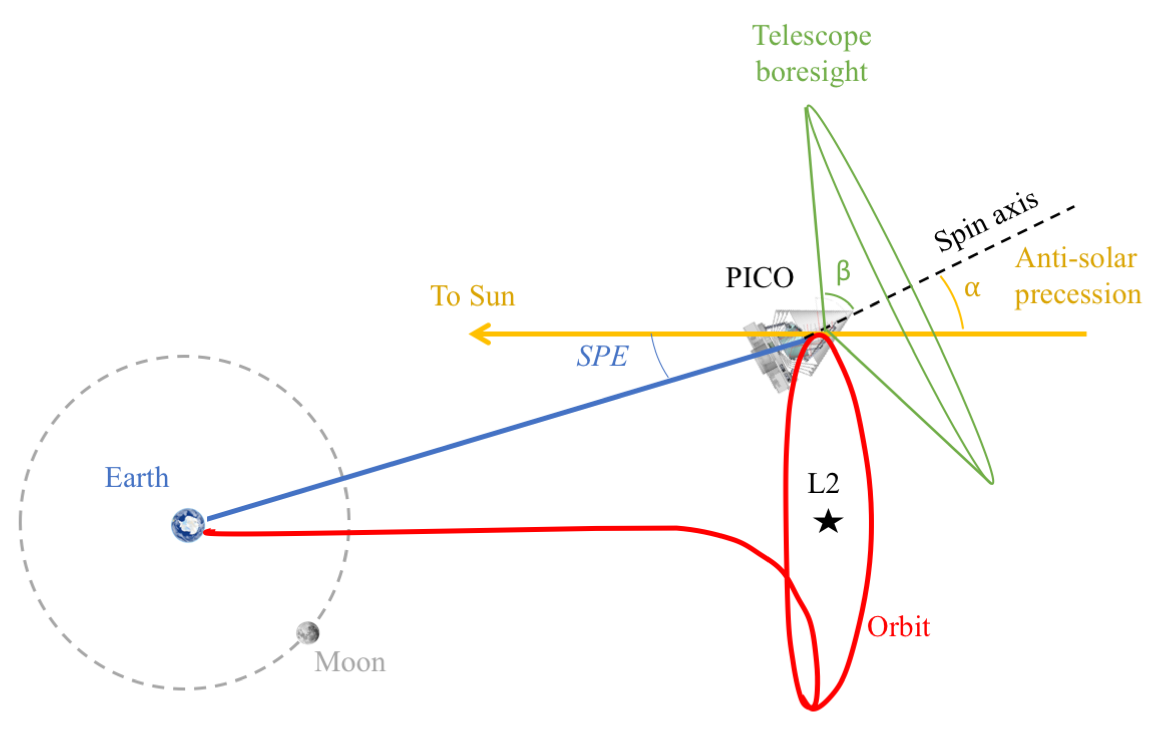
\includegraphics[width=2.5in]{figures/MissionDesignFigure.png} } }
\hspace{-0.6in}
\parbox{3.5in}{
\caption{\captiontext
PICO surveys the sky by spinning the instrument about the spacecraft's symmetry axis at 1~RPM. The telescope boresight is tilted by $\beta=69^{\rm{o}}$ from that axis. The symmetry axis precesses around the anti-sun direction with a period of 10~hours; $\alpha=29^{\rm{o}}$. Nearly 50\% of the sky is surveyed every two weeks. The entire sky is covered in 6 months. 
\label{fig:MissionDesignFigure}} }
%\end{center}
\vspace{-0.15in}
\end{figure}

Instrument data are compressed and stored on-board, then returned to Earth in daily 4-hr Ka-band science downlink passes (concurrent with science observations). High data-rate downlink to the Deep Space Network (DSN) is available from L2 using near-Earth Ka bands. We assumed a launch with the Falcon~9. Its capability for ocean recovery exceeds PICO's 2147\,kg total launch mass (including contingency) by a $50\,\%$ margin.

The PICO spacecraft bus is Class~B and is designed for a minimum lifetime of 5\,years in the L2 environment. Mission-critical elements are redundant. The aft end of the spacecraft (the ``de-spun module'') is comprised of six equipment bays that house standard components.  The instrument and V-grooves are mounted on bipods from the spacecraft's ``spun module,'' which contains the 4\,K cooler compressor and drive electronics, the sub-K cooler drive electronics, and the detector warm readout electronics. A motor drives the spun module at 1\,rpm. Only power and data (digital) lines pass between the spun and de-spun modules. Reaction wheels on the despun module cancel the angular momentum of the spun module and provide three-axis control.



